\begin{exercises} 

\item \label{Ez:9.5.1}   The vector and parametric forms of a line allow us to easily describe line segments in space. 

Let $P_1 = (1,2,-1)$ and $P_2 = (-2,1,-2)$, and let $\mathcal{L}$ be the line in $\R^3$ through $P_1$ and $P_2$ as in Activity \ref{A:9.5.2}.
\ba
	\item What value of the parameter $t$ makes $(x(t), y(t), z(t)) = P_1$? What value of $t$ makes $(x(t), y(t), z(t)) = P_2$?	
	\item What restrictions on the parameter $t$ describe the line segment between the points $P_1$ and $P_2$?
	\item What about the line segment (along the same line) from $(7,4,1)$ to $(-8,-1,-4)$?
	\item Now, consider a segment that lies on a different line:  parameterize the segment that connects point $R=(4,-2,7)$ to $Q=(-11,4,27)$ in such a way that $t = 0$ corresponds to point $Q$, while $t = 2$ corresponds to $R$.
	\ea
%\begin{figure}[h]
%\begin{center}
 %\includegraphics{figures/1_1_Ez1.eps}
 %\caption{A bungee jumper's height function.} \label{F:1.1.Ez1}
%\end{center}
%\end{figure}

\begin{exerciseSolution}
	\ba
	\item The line $\mathcal{L}$ can be expressed in vector form as $\vr(t) = \langle 1,2,-1\rangle + t\langle -3,-1,-1 \rangle$ and in parametric form as $x(t) = 1-3t$, $y(t) = 2-t$, and $z(t) = -1-t$. Note that $(x(0), y(0), z(0)) = P_1$ and $(x(1), y(1), z(1)) = P_2$. 
	\item If we restrict $t$ to be in the interval $[0,1]$ then our parameterization describes the line segment between the points $P_1$ and $P_2$.
	\item Here we note that $(x(-2), y(-2), z(-2)) = (7,4,1)$ and $(x(3), y(3), z(3)) = (-8,-1,-4)$. So restricting $t$ to lie in the interval $[-2,3]$ the parameterization describes the line segment from $(7,4,1)$ to $(-8,-1,-4)$.
	\item Since we want our parameterization be at $Q$ when $t=0$ and $R$ at $t=2$, we use the vector $\frac{1}{2}\overrightarrow{QR} = \frac{1}{2} \langle 15,-6,-20 \rangle$ as a direction vector for this line. So a parameterization of the segment that connects point $R=(4,-2,7)$ to $Q=(-11,4,27)$ in such a way that $t = 0$ corresponds to point $Q$, while $t = 2$ corresponds to $R$ is $x(t) = -11+\frac{15}{2}t$, $y(t) = 4-3t$, and $z(t) = 27-10t$.
	\ea
\end{exerciseSolution}

\item \label{Ez:9.5.2}   This exercise explores key relationships between a pair of lines.  Consider the following two lines:  one with parametric equations $x(s) = 4-2s$, $y(s) = -2 + s$, $z(s) = 1 + 3s$, and the other being the line through $(-4, 2, 17)$ in the direction $\vv = \langle -2, 1, 5 \rangle$.

%\begin{figure}[h]
%\begin{center}
 %\includegraphics{figures/1_1_Ez1.eps}
 %\caption{A bungee jumper's height function.} \label{F:1.1.Ez1}
%\end{center}
%\end{figure}

  \ba
  	\item  Find a direction vector for the first line, which is given in parametric form.
	\item  Find parametric equations for the second line, written in terms of the parameter $t$.
	\item  Show that the two lines intersect at a single point by finding the values of $s$ and $t$ that result in the same point.
	\item  Find the angle formed where the two lines intersect, noting that this angle will be given by the angle between their respective direction vectors.  
 	\item  Find an equation for the plane that contains both of the lines described in this problem. 
  \ea 


\begin{exerciseSolution}
  \ba
  	\item  The coefficients on the parameter provide a direction vector for the line, so a direction vector for the first line is $\langle -2, 1, 3 \rangle$. 
	\item  We are given a point and a direction, so a set of parametric equations for the second line is $x(t) = -4-2t$, $y(t) = 2+t$, and $z(t) = 17+5t$. 
	\item  A point that lies on both lines must simultaneously satisfy both sets of parametric equations. In other words, there must be a value of $s$ and a value of $t$ so that 
\begin{align*}
4-2s = -4-2t \\
-2 + s &=  2+t \\
1+3s &= 17+5t.
\end{align*}
The first and second equations are the same, both giving $s=t+4$. Substituting for $s$ in the third equation yields $t=-2$ and then $s=2$. This gives the point of intersection of the two lines as $(0,0,7)$. 
	\item  The direction vectors are $\vu = \langle -2, 1, 3 \rangle$ and $\vv = \langle -2, 1, 5 \rangle$. Then angle $\theta$ between $\vu$ and $\vv$ is given by 
\[\theta = \cos^{-1}\left(\frac{\vu \cdot \vv}{|\vu| |\vv|} \right) = \cos^{-1}\left(\frac{20}{\sqrt{14} \sqrt{30}} \right) \approx 12.6^{\circ}.\]
 	\item The plane will contain both direction vectors, so a normal to this plane is 
\[\vu \times \vv = \langle = \langle 2, 4, 0 \rangle.\]
The point $(-4,2,17)$ lies in this plane, so the equation of the plane that contains both lines is 
\[2(x+4)+4(y-2) = 0.\]
  \ea 
\end{exerciseSolution}

\item \label{Ez:9.5.3}   This exercise explores key relationships between a pair of planes.  Consider the following two planes:  one with scalar equation $4x - 5y + z = -2$, and the other which passes through the points $(1,1,1)$, $(0,1,-1)$, and $(4, 2, -1)$.

%\begin{figure}[h]
%\begin{center}
 %\includegraphics{figures/1_1_Ez1.eps}
 %\caption{A bungee jumper's height function.} \label{F:1.1.Ez1}
%\end{center}
%\end{figure}

  \ba
  	\item  Find a vector normal to the first plane.
	\item  Find the scalar equation for the second plane.
	\item  Find the angle between the planes, where the angle between them is defined by the angle between their respective normal vectors.
	\item  Find a point that lies on both planes.
	\item  Since these two planes do not have parallel normal vectors, the planes must intersect, and thus must intersect in a line.  Observe that the line of intersection lies in both planes, and thus the direction vector of the line must be perpendicular to each of the respective normal vectors of the two planes.  Find a direction vector for the line of intersection for the two planes.
	\item  Determine parametric equations for the line of intersection of the two planes. 
  \ea

\begin{exerciseSolution}
  \ba
  	\item  The coefficients of $x$, $y$, and $z$ tell us a normal vector for the first plane, so a normal vector for the first plane is $\langle 4, -5, 1 \rangle$. 
	\item  Let $P = (1,1,1)$, $Q = (0,1,-1)$ and $R = (4,2,-1)$. A normal vector for the plane will be 
\[\overrightarrow{PQ} \times \overrightarrow{PR} = \langle -1,0,-2 \rangle \times \langle 3, 1, -2 \rangle = \langle 2, -8, -1 \rangle.\]
Using the point $P$ gives us the scalar equation 
\[2(x-1) - 8(y-1) - (z-1) = 0.\]
	\item  The normal vectors are $\vn_1 = \langle 4, -5, 1 \rangle$ and $\vn_2 = \langle 2, -8, -1 \rangle$. The angle $\theta$ between the planes is the angle between $\vn_1$ and $\vn_2$ or 
\[\theta = \cos^{-1}\left(\frac{\vn_1 \cdot \vn_2}{|\vn_1| |\vn_2|} \right) = \cos^{-1}\left(\frac{47}{\sqrt{42} \sqrt{69}} \right) \approx 29.2^{\circ}.\]
	\item  Any point that lies on both planes must satisfy the two equations $4x - 5y + z = -2$ and $2(x-1) - 8(y-1) - (z-1) = 0$. If we choose a value for $z$, say $z=0$, then a point that lies on the intersection of the planes in the $x$-$y$ plane satisfies the equations $4x-5y=-2$ and $2x-8y=-7$. Using elimination (multiply both sides of the second equation by $-2$ and add corresponding sides of this new equation and the first) we find that $11y = 12$ or $y = \frac{12}{11}$. Then $x = \frac{19}{22}$. So the point $\left(\frac{19}{22}, \frac{12}{11}, 0\right)$ lies on both planes.  
	\item  A direction vector for the line of intersection of the two planes is 
\[\vn_1 \times \vn_2 = \langle 4, -5, 1 \rangle \times \langle 2, -8, -1 \rangle = \langle 13, 6, -22 \rangle.\]
	\item  Using the point on the intersection we found earlier, a set of parametric equations for the line of intersection of the two planes is 
\[x(t) = \frac{19}{22} + 13t, \ y(t) = \frac{12}{11} +6t, \ \text{ and } \ z(t) = -22t.\]. 
  \ea
\end{exerciseSolution}

\item \label{Ez:9.5.4}   In this problem, we explore how we can use what we know about vectors and projections to find the distance from a point to a
plane.

Let $p$ be the plane with equation $z=-4x+3y+4$, and let 
$Q = (4,-1,8)$.

% \begin{figure}[ht]
% \begin{center}
% \resizebox{!}{2.5in}{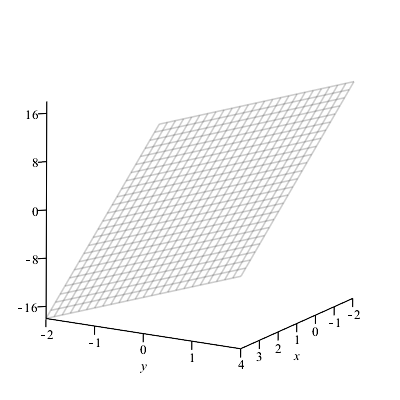
\includegraphics[trim=0cm 0.25cm 0cm 1.5cm, clip]{9_5_Point_to_plane}}
% \end{center}
% \caption{Graph of $z=-4x+3y+4$.}
% \label{F:9.5.Point_to_plane}
% \end{figure}
%crop graphics in animate trim=<left> <bottom> <right> <top>, add, clip with \includegraphics
	\ba
	\item Show that $Q$ does not lie in the plane $p$.
	\item Find a normal vector $\vn$ to the plane $p$.
	\item Find the coordinates of a point $P$ in $p$.
	\item Find the components of $\overrightarrow{PQ}$. Draw a picture to illustrate the objects found so far.
	\item Explain why $|\comp_{\vn} \overrightarrow{PQ}|$ gives the distance from the point $Q$ to the plane $p$. Find this distance.
	\ea

\begin{exerciseSolution}
	\ba
	\item Since $-4(4) + 3(-1) + 4 = -15 \neq 8$, the point $Q$ does not lie in the plane $p$.
	\item An equation of the plane is $4x-3y+z = 4$, so a normal vector to the plane $p$ is $\vn = \langle 4, -3, 1 \rangle$. 
	\item Choosing $x=y=0$ gives us a point $P = (0,0,4)$ in the plane $p$. 
	\item We have $\overrightarrow{PQ} = \langle 4, -1, 4 \rangle$. 
	\item The vector $\proj_{\vn} \overrightarrow{PQ}$ can be considered as a leg of a right triangle with hypotenuse $\overrightarrow{PQ}$. The length of this leg is the vertical distance from $Q$ to the plane, so its length, $|\comp_{\vn} \overrightarrow{PQ}|$, is the distance from the point $Q$ to the plane $p$. In our example we have
\[|\comp_{\vn} \overrightarrow{PQ}| = \frac{\overrightarrow{PQ} \cdot \vn}{|\vn|} = \frac{23}{\sqrt{26}}.\]
	\ea
\end{exerciseSolution}


\end{exercises}
\afterexercises
